\documentclass{PoS}
\newcommand{\as}{\\[14pt]}
\newcommand{\s}{\\[7pt]}
\newcommand{\is}{\\[2pt]}
\newcommand{\no}{\noindent}
\newcommand{\ka}{\hspace*{0.5cm}}
\newcommand{\ma}{\hspace*{1cm}}
\newcommand{\ga}{\hspace*{1.5cm}}
\newcommand{\li}{\left|}
\newcommand{\re}{\right|}
\newcommand{\const}{\text{const.}}
\newcommand{\z}{\text}
\newcommand{\terminal}[1]{\colorbox{black}{\textcolor{white}{{\fontfamily{phv}\selectfont \scriptsize{#1}}}}}
\newcommand{\plugin}[1]{\textit{\flq#1\frq}}
\newcommand{\ra}{$\rightarrow$ }
\definecolor{cadmiumgreen}{rgb}{0.0, 0.42, 0.24}
\newcommand{\itemfill}{\setlength{\itemsep}{\fill}}
\newcommand{\orderof}[1]{$\mathcal{O}\left(#1\right)$}
\newcommand{\fig}[2]{\begin{figure}\centering\includegraphics[height={#2}\textheight]{#1}\end{figure}}
\newcommand{\figc}[3]{\begin{figure}\centering\includegraphics[height={#2}\textheight]{#1}\caption{#3}\end{figure}}
\newcommand{\figp}[2]{\begin{figure}\centering\includegraphics[width={#2}\textheight, angle=-90]{#1}\end{figure}}
\newcommand{\figpc}[3]{\begin{figure}\centering\includegraphics[width={#2}\textheight, angle=-90]{#1}\caption{#3}\end{figure}}
\newcommand{\test}[1][bla]{#1}
\newcommand{\subfig}[4][0.45]{\begin{subfigure}{{#1}\textwidth}\centering
			\includegraphics[height={#3}\textheight]{#2}
			\caption{#4}\end{subfigure}}
\newcommand{\subfigp}[4][0.45]{\begin{subfigure}{{#1}\textwidth}\centering
			\includegraphics[width={#3}\textheight, angle=-90]{#2}
			\caption{#4}\end{subfigure}}

\usepackage[printonlyused]{acronym}
\usepackage{siunitx}
\usepackage{varioref}

\graphicspath{ {pics/} }
\makeatletter
\def\input@path{ {sections/} }
\makeatother

\title{Diamond Detector Technology: Status and Perspectives}
\ShortTitle{Diamond Detector Technology: Status and Perspectives}

\author{\speaker{Michael Reichmann}%
        \thanks{The full list of RD42 authors is provided in the appendix.}\\
       Eidgenoessische Technische Hochschule Zuerich (CH)\\
       E-mail: \email{michael.reichmann@cern.ch}}

\abstract{Here could be your abstract ;-)}

\FullConference{The European Physical Society Conference on High Energy Physics\\
         5-12 July\\
         Venice, Italy}

\makeindex
\begin{document}

%============= 1 =============
\section{Introduction}
The upgrade of the \ac{LHC} to the \ac{HL-LHC} from \SIrange{2023}{2025}{} \cite{hllhc} will push the luminosity limits even above the original design values of the \ac{LHC} and will therefore hopefully give us even more insights in the fundamental nature of the universe. In 2028 an instantaneous luminosity of \SI{5e34}{\per\centi\meter\squared\per\second} is aspired. This will be equivalent to a fluence of \SI{2e16}{n_{eq}\per \centi\meter^2} \cite{auzinger} for the innermost tracking layer at a distance of \SI{\sim30}{\milli\meter} from the interaction point. In this environment, pixel hit rates of \SI{3}{\giga\hertz\per\centi\meter^2} are expected. The current pixel detectors are designed to withstand \SI{\sim300}{\per\femto\barn} and thus the full detector would have to be replaced about every semester. This fact led to research and development of various radiation hard detector designs and materials.\\
Its large displacement energy and a high band gap of \SI{5.5}{\electronvolt} at \SI{305}{\kelvin} make diamond an excellent candidate for such a radiation tolerant detector which is why the RD42 Collaboration is investigating \ac{sc} and \ac{p} \ac{CVD} diamond as an alternative for precision tracking detectors for over two decades. In order to grow high quality detector grade diamonds, RD42 collaborates with industrial companies. All shown results are acquired with \ac{sc}\ac{CVD} diamonds produced by Element Six Technologies \cite{e6} and \ac{p}\ac{CVD} diamonds produced by II-VI Incorporated \cite{II6}. The two companies use propriety \ac{CVD} processes to fabricate their products. Both diamond types are grown on homo-epitaxial substrates with the difference that for \ac{sc}\ac{CVD} another \ac{sc}\ac{CVD} diamond is used as substrate and thus its size is limited to \SI{\sim0.25}{\centi\meter\squared}. However, for the \ac{p}\ac{CVD} a diamond powder can be used as a substrate whereby it can be grown to wafers of diameters up to \SI{6}{inch} \cite{felix}. In various studies it was found out that compared to corresponding silicon detectors, diamond is at minimum three times more radiation hard \cite{deboer}, has at least a two times faster charge collection \cite{pernegger} and its thermal conductivity is four times higher \cite{zhao}.\\
Due to the very high particle fluxes and radiation doses expected for the \ac{HL-LHC} it is very important to understand the behaviour of future detectors in this environment. The RD42 Collaboration has studied \ac{CVD} diamond detectors with irradiation doses up to \SI{2.2e16}{p\per\centi\meter^2}. In order to build even more radiation hard detectors a new technology - 3D detectors \cite{3D} - is investigated. The clever design of these detectors allows to heavily reduce the drift distance of the created charge carriers without reducing the total number of the created electron-hole pairs. Since the the signal behaviour of diamonds at high fluxes is uncertain, high rate studies are performed at \ac{PSI} with nearly \acp{MIP} and tunable particle fluxes from the order of \SI{1}{\kilo\hertz\per cm^2} up to the order of \SI{10}{\mega\hertz\per cm^2}.

%============= 1 =============
\section{Diamond Detectors at CERN}
It is essential for all modern collider experiments to have an online monitoring of the beam conditions. Since it is important to have these detectors as close as possible to the beam all of the four main experiments at the \ac{LHC} are using detectors with diamond sensors. ATLAS \cite{gorisek}, ALICE, CMS \cite{bartz} and LHCb \cite{domke} all make use of various \acp{BCM} and/or \acp{BLM} based on both \ac{CVD} type diamonds for live background estimations and luminosity measurements.\\
As an upgrade of the \ac{BCM} during the long shutdown in 2014 ATLAS installed the \ac{DBM}. Its purpose is to measure an instantaneous (bunch-by-bunch) luminosity and the bunch-by-bunch position of the beam spot. With its eight telescopes à three detector planes it adds tracking capability to the existing precise \ac{ToF} measurements of the eight pad detectors of the \ac{BCM}. The usage of state of the art pixel detectors based on the FE-I4b readout chip strongly increases the spatial resolution of the monitor and due to its projective geometry pointing towards the interaction region it also can distinguish particles coming from collisions and background \cite{dbm}. The telescopes whereof the sensors of two are made out silicon and the other six out of \ac{p}\ac{CVD} diamond are positioned symmetrically around the beam pipe on both sides of the interaction point and are shown in \vref{dbm}.
\begin{figure}
	\centering
	\begin{subfigure}{.66\textwidth}
		\centering
		\vspace*{.05\textheight}
		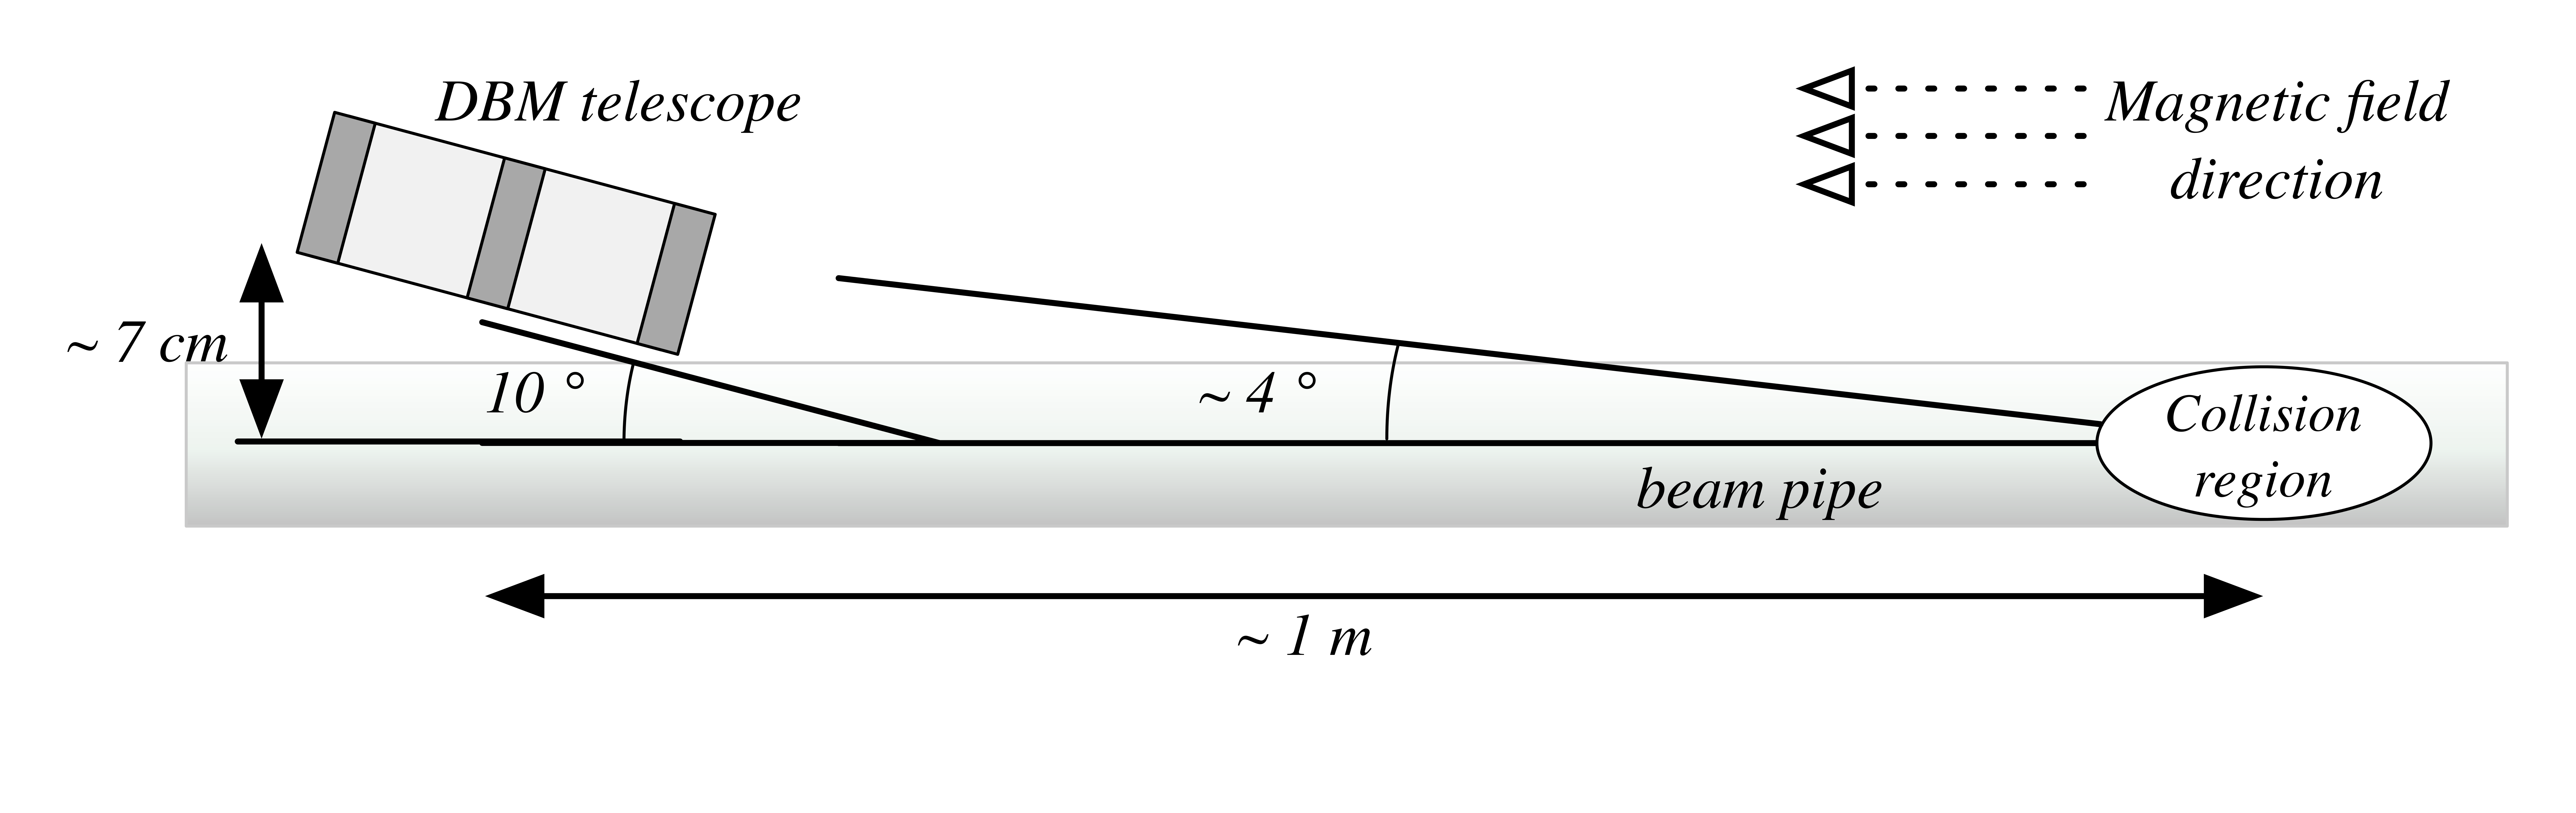
\includegraphics[height=.14\textheight]{dbm1.png}
		\vspace*{.02\textheight}
		\caption{positioning and alignment}
	\end{subfigure}
	\subfig[.33]{DBM2.png}{.23}{four mounted telescopes}
	\caption{\ac{DBM} telescope}
	\label{dbm}
\end{figure}



% ========== ACRONYMS ===========================
\newpage
\section*{List of Acronyms}
\begin{acronym}[Bash]
	\acro{PUC}{pixel unit cell}
	\acro{ROC}{readout chip}
	\acro{TBM}{token bit manager}
	\acro{UB}{ultra black}
	\acro{B}{black}
	\acro{CMS}{Compact Muon Solenoid}
	\acro{LHC}{Large Hadron Collider}
	\acro{HL-LHC}{High Luminosity LHC}
	\acro{CERN}{European Organization for Nuclear Research}
	\acro{DAC}{digital to analogue converter}
	\acro{ADC}{analogue to digital converter}
	\acro{LD}{last DAC}
	\acro{DTB}{digital test board}
	\acro{ATB}{analogue test board}
	\acro{ETH}{Eidgen{\"o}ssische Technische Hochschule}
	\acro{FPGA}{Field Programmable Gate Array}
	\acro{PSI}{Paul Scherrer Institut}
	\acro{HV}{high voltage}
	\acro{TTL}{Transistor-Transistor-Logic}
	\acro{PLL}{phase-locked loop}
	\acro{FIFO}{First In - First Out}
	\acro{HAL}{hardware abstraction layer}
	\acro{API}{application programming interface}
	\acro{GUI}{graphical user interface}
	\acro{CLI}{command line interface}
	\acro{DAQ}{data acquisition}
	\acro{CPU}{central processing unit}
	\acro{PG}{pattern generator}
	\acro{I2C}[I$^{2}$C]{Inter-Integrated Circuit}
	\acro{DUT}{device under test}
	\acro{TCP}{Transmission Control Protocol}
	\acro{TU}{trigger unit}
	\acro{COM}{centre of mass}
	\acro{PSB}{Proton Synchrotron Booster}
	\acro{PS}{Proton Synchrotron}
	\acro{SPS}{Super Proton Synchrotron}
	\acro{ALICE}{A Large Ion Collider Experiment}
	\acro{ATLAS}{A Toroidal LHC Apparatus}
	\acro{LHCb}{Large Hadron Collider beauty}
	\acro{LHCf}{ Large Hadron Collider forward}
	\acro{TOTEM}{TOTal Elastic and diffractive cross section Measurement}
	\acro{SUSY}{supersymmetry}
	\acro{HCAL}{hadronic calorimeter}
	\acro{ECAL}{electromagnetic calorimeter}
	\acro{CTR}{calibrate trigger reset}
	\acro{MIP}{minimum ionising particle}
	\acrodefplural{MIPs}{minimum ionising particles}
	\acro{PM}{photo multiplier}
	\acro{TLU}{trigger logic unit}
	\acro{PH}{pulse height}
	\acro{DC}{double column}
	\acro{DESY}{Deutsches Elektronen-Synchrotron}
	\acro{RAM}{Random-Access Memory}
	\acro{PCB}{printed circuit board}
	\acro{PLT}{Pixel Luminosity Telescope}
	\acro{RPC}{remote procedure calls}
	\acro{CVD}{Chemical Vapour Deposition}
	\acro{sc}{single-crystal}
	\acro{p}{poly-crystalline}
	\acro{BCM}{Beam Condition Monitor}
	\acrodefplural{BCMs}{Beam Condition Monitors}
	\acro{BLM}{Beam Loss Monitor}
	\acrodefplural{BLMs}{Beam Loss Monitors}
	\acro{DBM}{Diamond Beam Monitor}
	\acro{ToF}{time-of-flight}
	\acro{IP}{interaction point}
\end{acronym}

% ========== BIBLIOGRAPHY =======================
\newpage
\bibliographystyle{plain}
\bibliography{refs}

\end{document} 
